\chapter{Operational Amplifier}

\section{Design and Implementation}
The second stage of the design is the Operational Amplifier. This stage too, like the first stage uses a bipolar power supply of 2.5V and -2.5V. A two-stage Miller compensated op amp is designed and it is used as a Voltage Buffer for the OTA.
\subsection{Schematic}
The schematic of the Miller compensation op amp is as shown in the Figure.\ref{fig:OPAMP_Schematic}. The bias current to the differential pair is provided through the current mirror pair of $M_5$ and $M_8$. The bias current is controlled through the transistor $M_9$ whose gate voltage is provided by the voltage divider formed by the resistors $R_{b1}$ and $R_{b2}$. $C_C$ is the compensation capacitance between the two stages of the amplifier.
\begin{figure} [H]
\centering
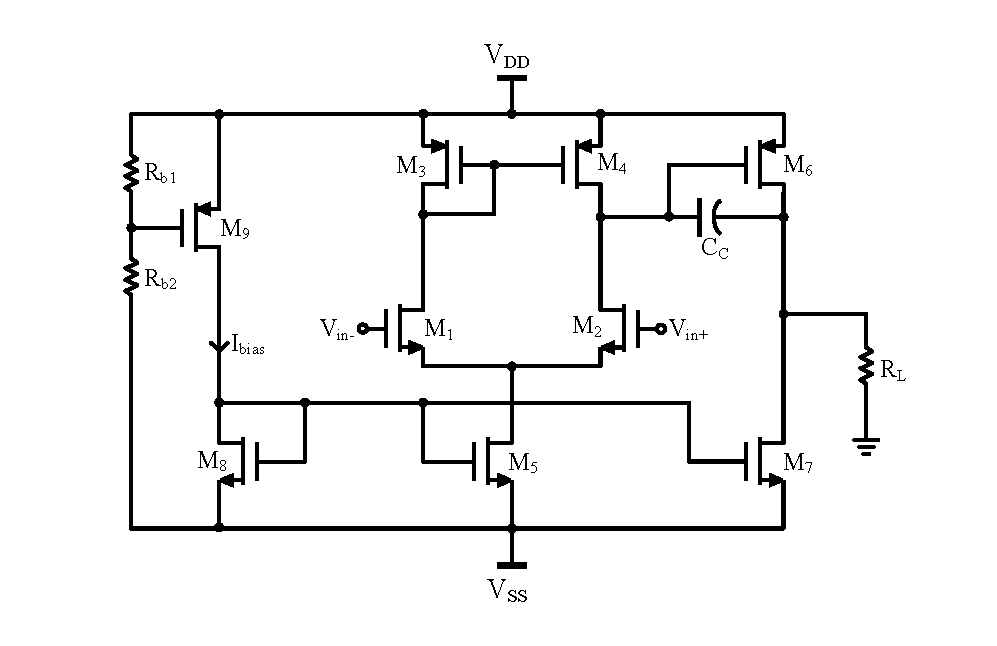
\includegraphics[scale=1]{Figures/Schematics/OPAMP_Vbias.pdf}
\caption{Schematic of the OPAMP Designed}
\label{fig:OPAMP_Schematic}
\end{figure}

The dimensions of the transistors are tabulated in Table.\ref{tab:OPAMP_dimensions}. One can easily recognize that the transistors at the output are large. This is designed so to make sure the op amp provides a very high current and thereby avoiding a common collector amplifier at the output of the op amp to amplify the output current. The compensation capacitance value is 50fF.

\begin{table} [H]
\centering
\begin{tabular}{@{}cccc@{}}
\toprule
Transistor			& Width				& Length			& Multiplier \\ \midrule
M1					& 5u				& 500n				& 2			\\
M2					& 5u				& 500n				& 2			\\ 
M3					& 30u				& 500n				& 1			\\
M4					& 30u				& 500n				& 1			\\ 
M5					& 2u				& 500n				& 1			\\
M6					& 85u				& 500n				& 55		\\ 
M7					& 50u				& 500n				& 48		\\
M8					& 2u				& 500n				& 1			\\ 
M9					& 700n				& 500n				& 1			\\
\bottomrule
\end{tabular}
\caption{Dimensions of the Transistors of the designed OPAMP}
\label{tab:OPAMP_dimensions}
\end{table}

\section{Test Setup}

\begin{figure} [H]
\centering
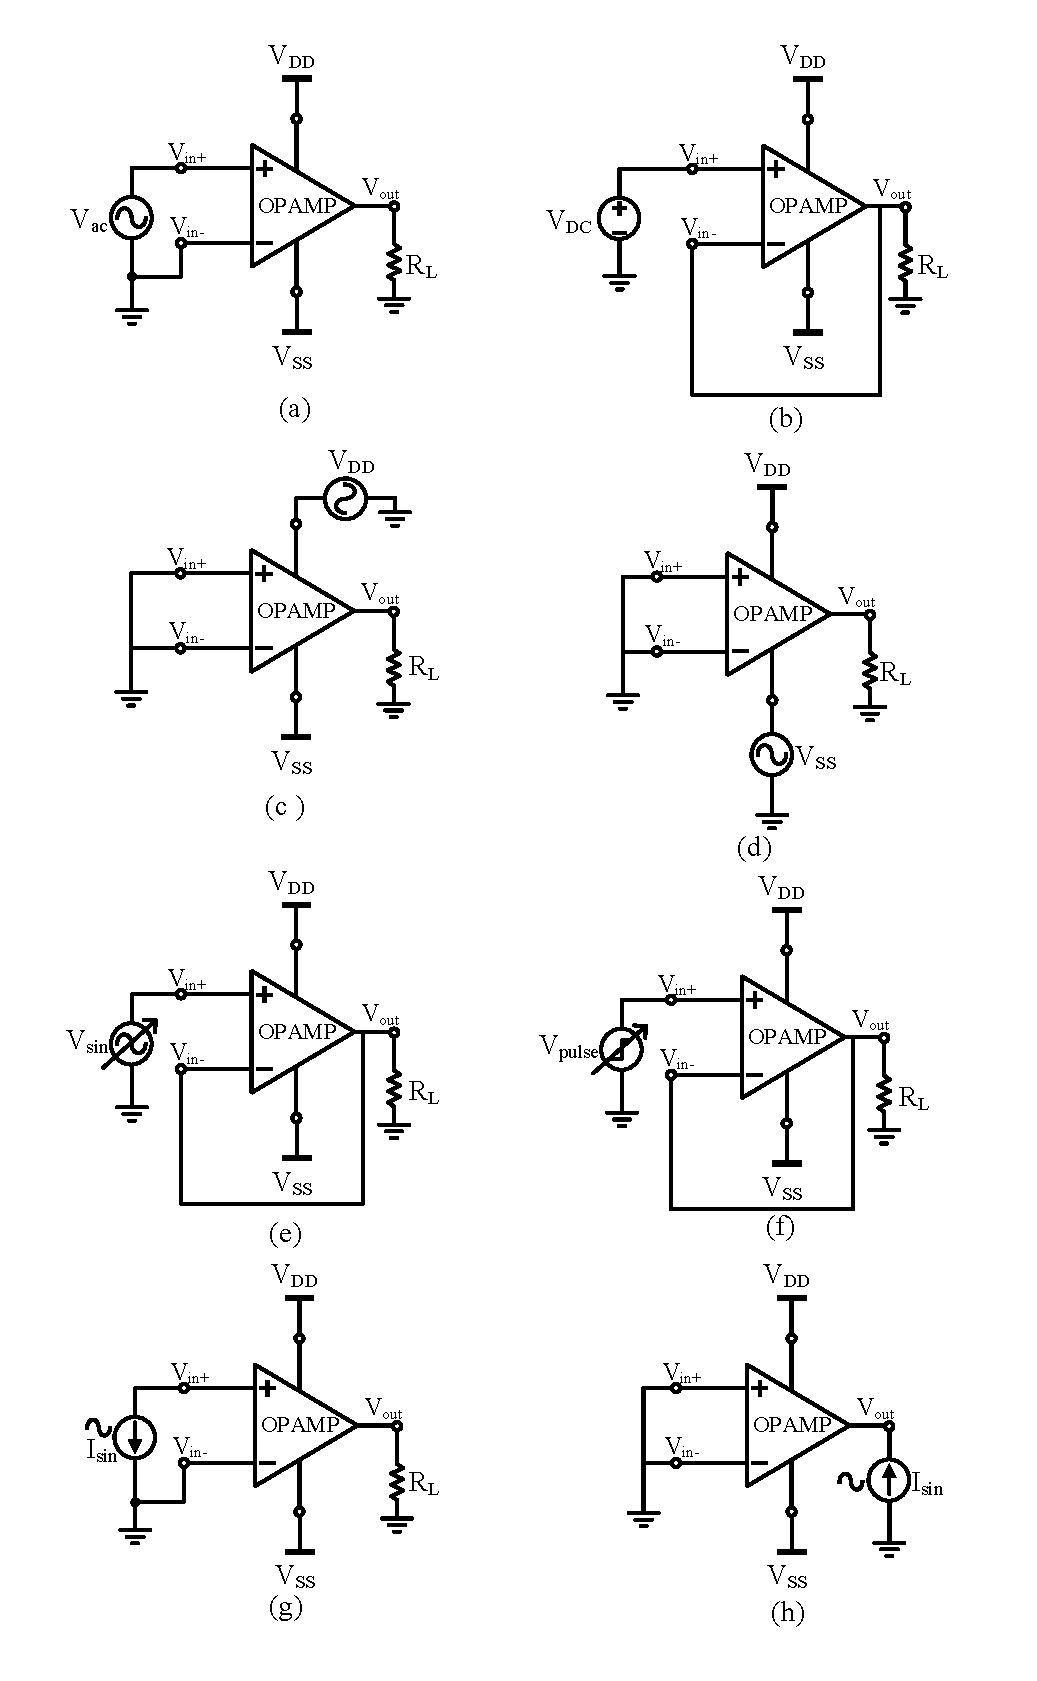
\includegraphics[scale=0.8]{Figures/Test_Benches/OPAMP_TB.pdf}
\caption{Test bench setup for OP AMP}
\label{fig:OPAMP_TB}
\end{figure}

\subsubsection{DC Analysis}


\subsubsection{AC Analysis}
The open loop gain and the gain bandwidth product are inarguably the most important parameters of an operational amplifier. Before the op amp was actually designed, these parameters were simulated with the help of an ideal op amp from the ahdlLib in Cadence. In order to have a stable system, i.e., an OTA with an OP AMP buffer in a cascade configuration, it is necessary to have the dominant poles far from each other. So that is the reason for the OTA to have a high bandwidth and correspondingly the OP AMP bandwidth can be adjusted so as to reach the specification and also to have a stable system.

The test bench used to measure these parameters is as shown in Figure.(a). The op amp is configured in an open loop. The DC biasing to the differential transistor pair is provided by the output of the OTA, which is centred around 0V. 

$V_{DD}$ = 2.5V; $V_{SS}$ = -2.5V; $V_{ac} magnitude $ = 1 V; $R_L$ = 50$\Omega$.

The plot of the open loop gain and the phase of the op amp is as shown in the Figure.\ref{fig:OPAMP_gain_pm_gbw}. The open loop gain of the op amp is 30.8dB. The gain bandwidth product is 6.2MHz and correspondingly the phase margin is $76.79^0$.

\begin{figure} [H]
\centering
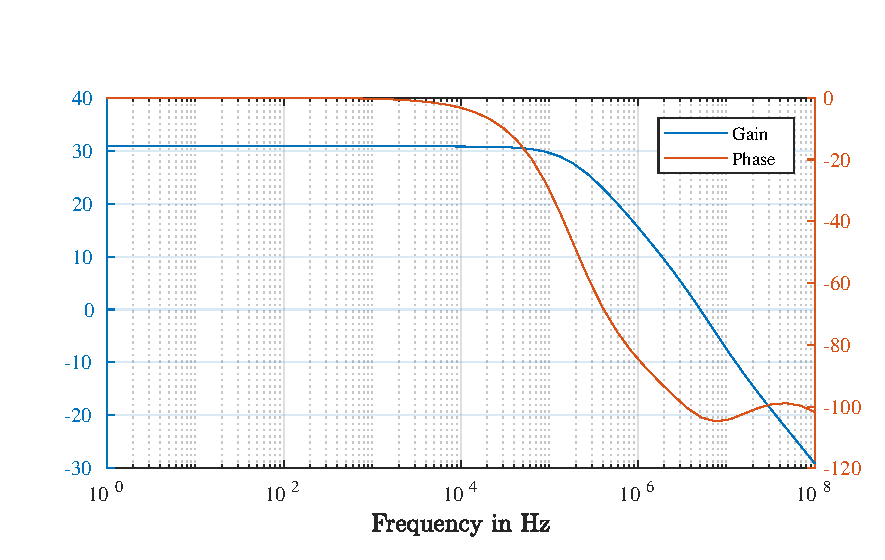
\includegraphics[scale=1]{Figures/Plots/OPAMP_Gain_PM.pdf}
\caption{OPAMP Plot of Gain and Phase vs Frequency}
\label{fig:OPAMP_gain_pm_gbw}
\end{figure}

The PSRR of the OTA in the first stage was in the range of $nA/V$ and hence neglibigle. However, the op amp designed exhibits a relatively high value of PSRR. This is due to the bulky transistors at the output stage. The test bench to measure the PSRR of the op amp is as shown in the Figure.(c). The one on the left is used to measure PSRR for a change in $V_{DD}$. And similarly, the one on the right side is used to measure PSRR for a change in $V_{SS}$.

$V_{DD}$ = 2.5V; $V_{SS}$ = -2.5V; $V_{ac} magnitude $ = 1 V; $R_L$ = 50$\Omega$.

The PSRR ($V_{DD}$) of the op amp is 30.96 uA/V, and PSRR ($V_{SS}$) is 130.96 uA/V. In the next chapter, it is seen that the assymetry in the two PSRR values doesn't affect the PSRR of the whole system.

The test bench to calculate the input impedance follows a similar concept to that of the OTA. i.e., a unity current source is connected to the non-inverting terminal of the op amp and the voltage at that terminal is measured which in turn is the magnitude of the input impedance of the op amp.

To have a stable system, it is important that input impedance of the second stage is higher than the output impedance of the first stage. Given that the output impedance of the OTA is generally high, the input impedance of the op amp becomes a very important parameter. And th input impedance is found to be 9.04M$\Omega$.

$V_{DD}$ = 2.5V; $V_{SS}$ = -2.5V; $I_{sin} magnitude $ = 1A.

Op amps are known to have zero or very low output impedance. Along with this theoretical fact, the op amp in this work is designed to retrieve very high currents, so it is expected to have a very low output impedance. The value of the output impedance is observed to be 4.167$\Omega$.

\subsubsection{Transient Analysis}
The test bench to perform the transient analysis is as shown in the Figure.(e). The op amp is connected in a negative feedback configuration so as to analyse its behavior as a voltage buffer.

$V_{DD}$ = 2.5V; $V_{SS}$ = -2.5V; $V_{sin} amplitude $ = 1.5V; $frequency$ = 1MHz; $R_L$ = 50$\Omega$.

The of input voltage and output voltage with respect to time is as shown in the Figure.\ref{fig:OPAMP_Vout}. The output follows the input only with a very small delay.

\begin{figure} [H]
\centering
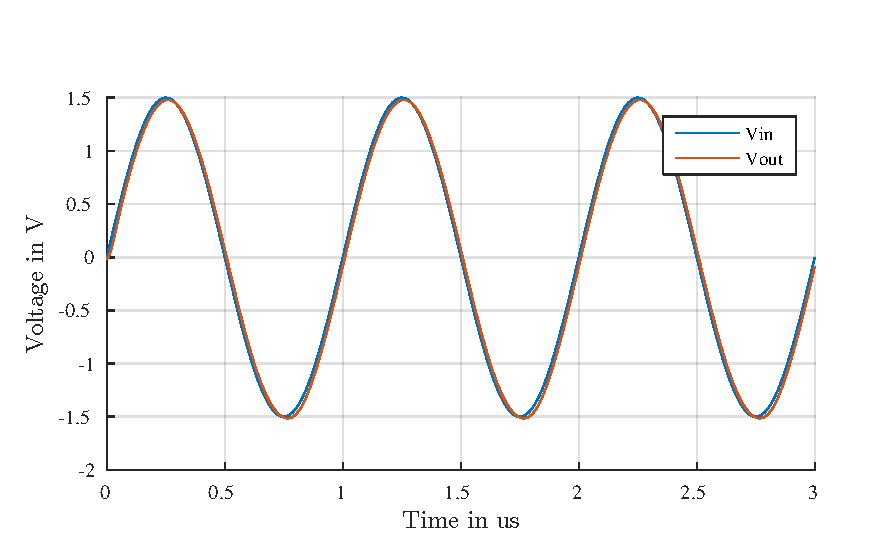
\includegraphics[scale=1]{Figures/Plots/OPAMP_Buffer.pdf}
\caption{OPAMP Plot of Output Voltage vs time}
\label{fig:OPAMP_Vout}
\end{figure}

The output current of the op amp is effectively the current flowing through the load resistor $R_L$. The plot of current versus time is as shown in the Figure.\ref{fig:OPAMP_Iout}. The current is $180^0$ out of phase with the voltage and it ranges from -30mA to 30mA for a 50$\Omega$ load and 3V peak to peak input voltage. 

\begin{figure} [H]
\centering
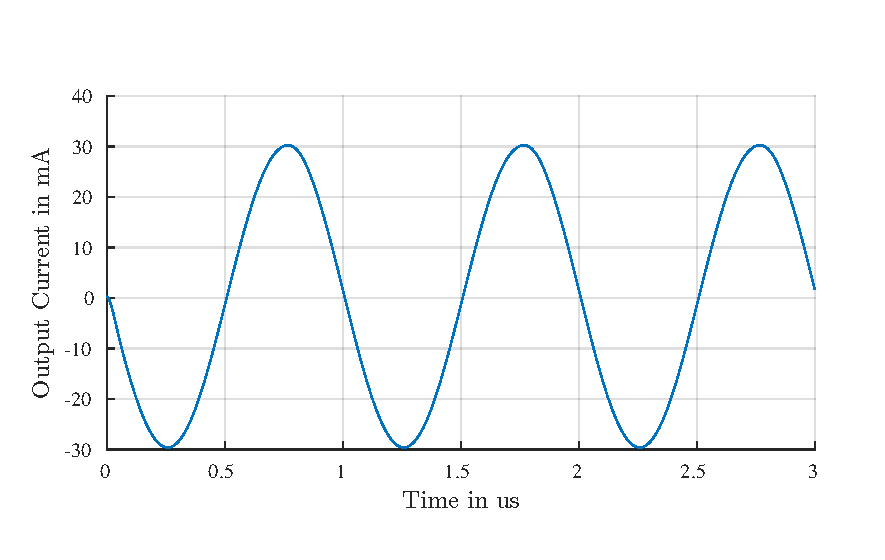
\includegraphics[scale=1]{Figures/Plots/OPAMP_Iout.pdf}
\caption{OPAMP Plot of Ourput Current vs time}
\label{fig:OPAMP_Iout}
\end{figure}

\section{Summary}

The values of all the parameters of the op amp discussed so far have been tabulated in Table.\ref{tab:OPAMP_Results}
\begin{table} [H]
\centering
\begin{tabular}{@{}cc@{}}
\toprule
Parameter					& Value				\\ \midrule
Open Loop Gain				& 30.8 dB			\\
Gain Bandwidth Product		& 6.2 MHz			\\
Phase Margin				& 76.79				\\
ICMR (min)					& -2.19 V			\\
ICMR (max)					& 2.089 V			\\
Output Current (max)		& -29.6 mA			\\
Output Current (min)		& 30.28 mA			\\
Output Voltage Swing		& -2.19 .. 2.323 	\\
Slew Rate					& 10 V/us			\\
PSRR (VDD)					& 30.96 uA/V		\\
PSRR (VSS)					& 138.8 uA/V		\\
Input Impedance				& 9.04 MOhms		\\
Output Impedance			& 4.167 Ohms		\\
\bottomrule
\end{tabular}
\caption{Simlation Results of the OPAMP}
\label{tab:OPAMP_Results}
\end{table}